% =============================================================================
% International Journal of Advanced Science and Engineering (IJASE)
% Mahendra Publications — Original Research Article
% Format per IJASE Guide for Authors:
%   - A4, 12 pt standard font, double spacing, wide (3 cm) margins
%   - NO full justification (ragged right), every paragraph indented
%   - Numbered sections (1, 1.1, 1.1.1); Results and Discussion combined
%   - Conclusions <= 100 words; Abstract 100-150 words
%   - References numbered in order of first appearance, [n] in text
%   - Tables and figures each on a separate page at the END of the manuscript
% =============================================================================
\documentclass[12pt,a4paper]{article}

\usepackage[a4paper,margin=3cm]{geometry}      % IJASE: wide 3 cm margins
\usepackage{times}                              % standard serif font
\usepackage[T1]{fontenc}
\usepackage[utf8]{inputenc}
\usepackage{setspace}
\usepackage{indentfirst}                         % indent first paragraph of each section
\usepackage{amsmath,amssymb}
\usepackage{booktabs}
\usepackage{array}
\usepackage{graphicx}
\usepackage{caption}
\usepackage[hidelinks]{hyperref}
\usepackage{url}
\usepackage{tikz}
\usetikzlibrary{arrows.meta,positioning,calc}
\usepackage{pgfplots}
\pgfplotsset{compat=1.17}

\captionsetup{font=small,labelfont=bf,labelsep=period}

% Numbered headings: 1.  1.1  1.1.1
\renewcommand{\thesection}{\arabic{section}.}
\renewcommand{\thesubsection}{\arabic{section}.\arabic{subsection}}
\renewcommand{\thesubsubsection}{\arabic{section}.\arabic{subsection}.\arabic{subsubsection}}

\title{\textbf{Calibrated Conviction: A Multi-Source Ensemble that Knows
When Not to Predict in the Indian Equity Market}}

\author{
Anandkumar Pardeshi\,$^{a,*}$ \quad and \quad Sujata Deshmukh\,$^{b}$\\[0.6em]
\small $^{a}$Department of Computer Science and Engineering,\\
\small Fr.\ C.\ Rodrigues Institute of Technology, Vashi, Navi Mumbai 400703, India\\[0.3em]
\small $^{b}$Department of Computer Engineering,\\
\small Fr.\ C.\ Rodrigues Institute of Technology, Vashi, Navi Mumbai 400703, India\\[0.4em]
\small $^{*}$Corresponding author. E-mail: \texttt{anand.pardeshi@fcrit.ac.in};\\
\small Tel.: +91-22-2768-0000
}
\date{}

% =============================================================================
\begin{document}
\maketitle

% IJASE: ragged right (no constant right margin); keep paragraph indentation.
\raggedright
\setlength{\parindent}{1.27cm}
\setlength{\parskip}{0pt}
\doublespacing

% ---------- Abstract (100-150 words, no references) ----------
\begin{abstract}
\normalsize\noindent
Many published equity-prediction systems advertise directional accuracies that
collapse once their probabilities are calibrated and realistic transaction costs
are charged. We went the other way, asking what a forecaster in an emerging market
can be trusted to deliver.
Eight years of National Stock Exchange of India data give a blunt answer:
next-period single-name direction is essentially unpredictable, and a
cross-sectional gradient-boosted model confirms it at 50.1\% out-of-sample
accuracy---no better than the upward drift. The value lies elsewhere:
a three-stage procedure cuts the hybrid ensemble's expected calibration error from
0.35 to 0.05, and a conviction-gated swing signal,
at a thirty-trading-day horizon, lifts the realized hit-rate to 60.6\% against a
58.1\% base rate while firing on only 5.7\% of observations and beating it in four
of five test years. Every figure here is a measured walk-forward statistic.
\end{abstract}

\noindent\textbf{Keywords:} Equity forecasting; Probability calibration;
Conformal prediction; Ensemble learning; Conviction gating

% ---------- Highlights (IJASE mandatory; 3-5 bullets, <= 85 chars each) ----------
\vspace{0.6em}
\noindent\textbf{Highlights}
\begin{itemize}\setlength{\itemsep}{0pt}
  \item Daily single-name NSE direction carries no edge beyond drift (50.1\% OOS).
  \item A three-stage calibration cuts expected calibration error from 0.35 to 0.05.
  \item A conviction gate lifts the 30-day hit-rate to 60.6\% vs a 58.1\% base rate.
  \item The high-conviction bucket beats the base rate in four of five test years.
  \item Every displayed statistic is a measured walk-forward result, not a fit.
\end{itemize}

% =============================================================================
\section{Introduction}
% =============================================================================

The trouble with much of the machine-learning-for-finance literature is not that
the models fail. It is that they seem to succeed. Directional accuracies of
60--70\% turn up regularly, but they tend not to survive a few basic checks: are
the reported probabilities calibrated, does the evaluation respect the order of
time, and are realistic Indian transaction costs charged on every round trip
\cite{r_liu}? We applied those checks to our own platform, and the comfortable
numbers evaporated. What follows is an account of what was left once they did,
and of the engineering that made the remainder worth trusting.

Our setting is the National Stock Exchange of India (NSE). It is a market driven
by Foreign and Domestic Institutional Investor (FII/DII) flows and by a large
retail base that reacts to news in both English and Hindi. Earlier multi-source
studies report that fusing price, news and order-flow can raise accuracy above
single-source baselines \cite{r_nti,r_long,r_fu}, and hybrid sentiment-indicator
architectures have been proposed for movement prediction \cite{r_moodi,r_farhadi}.
What that body of work rarely asks is whether the probabilities it produces can be
believed. The efficient-market hypothesis \cite{r_fama} says that short-horizon
direction for liquid large-caps ought to be close to unpredictable; our own results
agree. For an applied system, then, the job is not to argue the limit away but to
work sensibly within it.

We rebuilt the project around four aims: to bring financial metrics, multilingual
sentiment, FII/DII flows and macroeconomic state into a single feature space
(Section~2.1--2.3); to make the ensemble's probabilities calibrated rather than
merely confident, since a confidence score you cannot trust is worse than none
(Section~2.4--2.5); to build a decision layer that stays silent by default and acts
only above a conviction threshold validated out of sample, with distribution-free
intervals attached (Section~2.6--2.7); and to keep the whole thing explainable and
able to audit itself (Section~2.8--2.9). The empirical core in Section~3 is modest
about what it claims and open about where it fails.

% =============================================================================
\section{Materials and Methods}
% =============================================================================

\subsection{Multi-source data ingestion}

Let $t$ index NSE trading days. We align four streams on a common daily grid:
adjusted OHLCV bars via \texttt{yfinance}; news and social text from NewsAPI,
Google News RSS (English and Hindi), the \texttt{gnews} library and Economic Times
feeds, behind a URL-level domain filter that drops non-financial sources, such as
the software registries the word ``Reliance'' would otherwise match; FII and DII
daily net flows in INR crore, lagged one session so nothing leaks from the future;
and macroeconomic state---the India VIX, INR/USD, Brent crude and gold as clipped
log-returns, with NIFTY-relative strength and beta.

\subsection{Feature engineering}

Each ticker-day is described by a vector of roughly forty stationary inputs,
organized into ten groups: multi-horizon returns (1--20 days); volatility
(realized and normalized ATR); momentum and oscillators (Wilder RSI, Bollinger
Band \%B in Eq.~\eqref{eq:rsi}, the 12/26/9 MACD line and histogram, Williams \%R);
volume (volume ratio, on-balance-volume slope, Chaikin Money Flow); trend strength
(Average Directional Index, Aroon, 9/21/50 EMA slopes); lagged divergence flags;
chart-pattern distance-to-target; FinBERT sentiment; lagged FII/DII flows; macro
returns; and NIFTY-relative strength and beta. Two details guard against leakage:
every divergence flag is shifted one period before comparison, so no feature sees
its own future, and each column is winsorized and scaled on the training fold
alone.

\begin{equation}
\mathrm{RSI}_{14}(t)=100-\frac{100}{1+\mathrm{RS}_{14}(t)},\qquad
\mathrm{BB}_{\%B}(t)=\frac{C_t-\mathrm{LB}(t)}{\mathrm{UB}(t)-\mathrm{LB}(t)+\varepsilon}
\label{eq:rsi}
\end{equation}

\subsection{FinBERT sentiment pipeline}

A FinBERT pipeline \cite{r_araci} (the \texttt{ProsusAI/finbert} checkpoint) scores
each headline and returns a raw polarity $\tilde{s}=p_+-p_-$. FinBERT tends to
over-assign the neutral class on short headlines, so a curated layer of about sixty
Indian-market bullish and bearish terms (``upper circuit'', ``promoter pledge'',
``SEBI ban'') fixes the high-precision cases. Hindi articles are
machine-translated first, since the model is English-only. We take the daily ticker
score as a source-weighted mean, and a separate large-language-model layer rates
novelty and materiality to build a news-alpha term.

\subsection{Heterogeneous ensemble and leak-free stacking}

We train five base learners per ticker. XGBoost \cite{r_xgboost} and LightGBM
\cite{r_lightgbm} run shallow and L1/L2-regularized for the short per-ticker
window; CatBoost \cite{r_catboost} joins them; a multi-task LSTM--GRU network
carries three heads (return, direction under binary cross-entropy, and a soft-plus
volatility head); and ARIMA and Prophet sit in as fading statistical priors.
Out-of-fold (OOF) predictions come from a purged, embargoed, expanding-window
scheme: a five-day purge and embargo separate each validation block from its
training window, so lagged-return features cannot bleed across the boundary---the
standard precaution for financial cross-validation \cite{r_prado}. The OOF matrix
then feeds a Ridge meta-learner \cite{r_wolpert},
\begin{equation}
\hat{s}^{\mathrm{stack}}_t=\boldsymbol{\beta}^{\!\top}\mathbf{z}_t+\beta_0,\qquad
[\boldsymbol{\beta};\beta_0]=(\tilde{\mathbf Z}^{\!\top}\tilde{\mathbf Z}+\lambda\mathbf I)^{-1}\tilde{\mathbf Z}^{\!\top}\mathbf y ,
\label{eq:stack}
\end{equation}
and because it is built on out-of-fold rows, leakage has nowhere to enter. A
pre-trained cross-sectional LightGBM is let in at a small weight, but only if its
own OOF accuracy clears a gate set just above chance.

\subsection{Three-stage probability calibration}

No single change mattered more. An earlier version of the system was badly
miscalibrated: it reported an average up-probability near 0.80 against a realized
base rate near 0.48, an expected calibration error (ECE) of roughly 0.35, and a
Brier score worse than a constant forecast. The cause was twofold. An isotonic
calibrator fitted on the tree-average OOF distribution had been applied to the
Ridge meta-output, a different distribution; and the final convex blend of two
individually calibrated probabilities was never recalibrated, even though a convex
combination of calibrated forecasts is not itself calibrated. The fix has three
stages: an isotonic regression \cite{r_zadrozny} fitted on the tree-average OOF
predictions and applied to the matching tree-average test predictions; a
validation-fitted Platt scaler \cite{r_platt} on the recurrent network's sigmoid
output; and, after the $0.60$/$0.40$ blend, a logistic recalibration on the
held-out validation fold that pulls a low-skill model back toward the base rate
rather than letting it claim confidence it has not earned. Calibration is measured
by ECE over ten bins and the Brier score \cite{r_brier}, and the same transform is
applied to the live inference row, so the probability a user sees sits on the same
corrected scale.

\subsection{Conformal prediction intervals}

Every point forecast carries a distribution-free interval. Two quantile XGBoost
regressors are trained at the 0.10 and 0.90 levels, and the split-conformal
half-width is the finite-sample-corrected quantile of absolute residuals, on a
held-out fold disjoint from where the band is applied
\cite{r_romano,r_angelopoulos}. Under exchangeability the interval has a marginal
coverage guarantee; in practice, serial dependence means the coverage we observe is
just that---an observation, not a guarantee.

\subsection{Conviction-gated swing-direction signal}

Since next-day direction proved unpredictable (Section~3.1), the signal we trade
aims at a longer, more tractable question: over the next thirty trading
days---roughly six calendar weeks---is a name more likely than not to be higher
than today, and is the setup convincing enough to act on? A cross-sectional
logistic model takes nine point-in-time features: 12-1 month
momentum \cite{r_jt}, intermediate-term and quarterly returns, a five-day reversal,
distance from the 200-day average, a golden-cross flag, RSI, realized volatility,
and an above-average flag. We evaluate it with an embargoed, expanding-window
walk-forward over 2018--2026. Two design choices keep it disciplined. It is
long-or-neutral only, because confident single-name shorts get run over by the
upward drift; and it fires only above a conviction threshold $\tau^{\star}$, set
out of sample as the lowest threshold whose fired bucket still reaches a target
precision while firing on at least 5\% of observations. The expected hit-rate we
report is the \emph{measured} walk-forward precision of that bucket, not an
in-sample fit---the whole point of what we call the ``honesty contract''.

\subsection{Explainability, risk controls and self-audit}

For attribution we run TreeSHAP \cite{r_lundberg} on the gradient-boosted learner,
read alongside the swing model's own coefficients and the gain importances of the
cross-sectional model (Section~3.4). Market regime is labelled by the Hurst
exponent \cite{r_hurst}, gated by the Average Directional Index. At the portfolio
level, signal weights follow a mean-variance rule,
$\mathbf w^{\star}\propto\boldsymbol\Sigma^{-1}\mathbf{IC}$ \cite{r_grinold}, sized
by a quarter-Kelly rule \cite{r_kelly} under 5\% per-name, 30\% sector and 15\%
volatility caps. The cost side is charged in full---brokerage, securities
transaction tax, exchange and SEBI fees, stamp duty, 18\% GST and a square-root
market-impact term---and a gate throws out any signal whose expected alpha falls
below twice the round-trip cost. Every prediction lands in an append-only ledger,
and a live monitor halts emission whenever the sixty-day Sharpe stays negative, so
the system steps aside instead of trading through a regime it cannot handle.

\subsection{Datasets, baselines and evaluation}

The universe is the NSE large-cap set (54 names after liquidity screening), 28~May
2018 to 27~May 2026. The cross-sectional study uses a ten-year panel of 131{,}809
ticker-days with a five-day excess-return-over-NIFTY target; the swing study uses
91{,}471 labelled ticker-days, of which 50{,}272 are strictly out of sample. We
chose hard baselines on purpose: the upward base rate itself (the toughest
benchmark a drifting market offers), an always-majority-class rule, and an
uncalibrated version of our own ensemble. Metrics are directional accuracy, ECE
over ten bins, the Brier score, and walk-forward precision and coverage. Everything
runs on commodity hardware with freely available data.

% =============================================================================
\section{Results and Discussion}
% =============================================================================

\subsection{The limits of daily directional prediction}

Our first result is also our most important, and it is negative. A cross-sectional
LightGBM, trained on 71 engineered features across 131{,}809 ticker-days with a
five-day excess-return target and a date-based out-of-fold scheme that blocks
per-ticker leakage, landed at an out-of-sample directional accuracy of
50.09\%---a coin toss, indistinguishable from the upward drift. Why so flat? No
single feature accounts for more than 3.4\% of total gain, and the importance
distribution is nearly level, so there is no concentrated structure to learn at
this horizon. We chased the same null four more ways---per-ticker ensembling, a
cross-sectional logistic, a LightGBM-with-reversal model, and trend- and
regime-gated variants---and short-horizon single-name accuracy never climbed above
the base rate. For liquid large-caps this is exactly what the efficient-market
hypothesis predicts \cite{r_fama}, and we say so plainly, because tuning a number
until it looks good is how the literature's inflated accuracies arise.

\subsection{Calibration: from overconfidence to honesty}

If a model cannot beat the base rate, the least it can do is admit as much---and the
three-stage calibration of Section~2.5 was the biggest improvement we made.
Table~\ref{tab:headline} and Figure~\ref{fig:calib} show what changed. Before the
fix, the reliability curve ran well below the diagonal: up-probabilities clustered
near 0.80 while the realized frequency hovered around 0.50, the ECE sat near 0.35,
and the Brier score came in above the constant-forecast $p(1-p)$. Afterward the
curve hugs the diagonal, the ECE drops to roughly 0.05, and the average reported
probability settles near the base rate. Accuracy barely moved---which is the point:
calibration and discrimination are orthogonal, so we gave up false confidence, not
signal. A miscalibrated 80\% drives systematic over-betting under any
confidence-proportional sizing rule; getting the probabilities right makes the rest
safe to size on.

\subsection{A conviction gate turns a weak edge into a usable one}

The payoff is small but real, and it shows up at a longer horizon. Over thirty
trading days the conviction-gated signal of Section~2.7 stays silent 94\% of the
time---it fires on just 5.65\% of observations---and when it fires it is right
60.63\% of the time against a 58.05\% base rate. The $+2.6$-point lift is modest
but measured strictly out of sample across 50{,}272 observations, and it is stable.
Table~\ref{tab:swing} shows the fired bucket beating
its own yearly base rate in four years out of five: by $+10.8$ points in 2025 and
$+7.4$ in the 2026 drawdown, when the base rate itself had slipped below 50\%. The
lone losing year, 2024, cost $2.4$ points. The telling number is the raw signal's
global ROC AUC: 0.47, below chance as a ranker. The edge is not in how the signal
orders all names but in the extreme high-conviction tail---which is why a
conviction \emph{gate}, not a ranking, is the right way to use a weak signal,
something the AUC alone would have buried.

\subsection{Attribution, intervals and self-audit}

Being a linear classifier, the swing model wears its attribution on its sleeve. The
standardized coefficients (Table~\ref{tab:swing}, lower panel) put realized
twenty-day volatility first, then quarterly return and 12-1 momentum, both with
negative signs, and no coefficient exceeds 0.14. That mirrors the flat
cross-sectional importances and says the same thing: the edge is diffuse, not the
work of any single factor. Inside the per-ticker ensemble, TreeSHAP and the FinBERT
score rank sentiment and FII flows among the non-redundant contributors
\cite{r_nti,r_long}. The conformal intervals held empirical coverage close to the
nominal 80\%, the small misses tracing to the serial dependence that breaks exact
exchangeability \cite{r_angelopoulos}. The signal earned its keep mostly in
trending Hurst regimes and least in mean-reverting ones---which is why the live
monitor's suspension on a negative sixty-day Sharpe matters: under costs two to
three times the usual ten-basis-point assumption, the system stands down where its
evidence says the edge is gone.

\subsection{Limitations}

A few caveats remain. The evidence is one market and one eight-year window that, on
balance, trended; multi-regime, multi-market replication is future work. The swing
edge, though stable, is small and concentrated, so its value after costs depends on
execution quality and the 5--6\% firing rate. The cross-sectional null is specific
to liquid large-caps and end-of-day data, and sentiment coverage thins in sectors
with specialized jargon---left for later work.

% =============================================================================
\section{Conclusions}
% =============================================================================

An honest evaluation is unambiguous: next-day single-name direction on NSE
large-caps is unpredictable beyond drift, at 50.1\% out of sample. The value sits
elsewhere: a three-stage calibration cuts the expected calibration error from 0.35
to 0.05, and a conviction gate lifts the thirty-day hit-rate to 60.6\% against a
58.1\% base rate, beating it in four of five years while abstaining 94\% of the
time. A system that knows when to keep quiet is worth more than one that claims too
much.

% =============================================================================
\section{Acknowledgements}
% =============================================================================

The authors thank the maintainers of \texttt{yfinance}, HuggingFace Transformers,
XGBoost, LightGBM, CatBoost and SHAP. No external funding was received.

% =============================================================================
\section{References}
% =============================================================================
\renewcommand{\refname}{}
\vspace{-2\baselineskip}
\begin{singlespace}
\begin{thebibliography}{99}
\setlength{\itemsep}{0pt}
\setlength{\parskip}{0pt}

\bibitem{r_liu}
Liu, C., Arulappan, A., Naha, R., Mahanti, A., Kamruzzaman, J., Ra, I.H., 2024.
Large language models and sentiment analysis in financial markets: a review,
datasets, and case study. IEEE Access, 12, 134041--134061.

\bibitem{r_nti}
Nti, I.K., Adekoya, A.F., Weyori, B.A., 2021. A novel multi-source
information-fusion predictive framework based on deep neural networks for accuracy
enhancement in stock market prediction. Journal of Big Data, 8, 17.

\bibitem{r_long}
Long, W., Gao, J., Bai, K., Lu, Z., 2024. A hybrid model for stock price prediction
based on multi-view heterogeneous data. Financial Innovation, 10, 48.

\bibitem{r_fu}
Fu, K., Zhang, Y., 2024. Incorporating multi-source market sentiment and price data
for stock price prediction. Mathematics, 12, 1572.

\bibitem{r_moodi}
Moodi, F., Jahangard-Rafsanjani, A., Zarifzadeh, S., Zare Chahooki, M.A., 2024.
Fusion of technical indicators and sentiment analysis in a hybrid framework of deep
learning models for stock price movement prediction. IEEE Access, 12,
195696--195709.

\bibitem{r_farhadi}
Farhadi, A., Zamanifar, A., Alipour, A., Taheri, A., Asadolahi, M., 2025. A hybrid
LSTM-GRU model for stock price prediction. IEEE Access, 13, 117594--117618.

\bibitem{r_fama}
Fama, E.F., 1970. Efficient capital markets: a review of theory and empirical work.
Journal of Finance, 25, 383--417. \mbox{DOI: 10.2307/2325486.}

\bibitem{r_araci}
Araci, D., 2019. FinBERT: financial sentiment analysis with pre-trained language
models. arXiv:1908.10063 [Internet]. [cited 2026 May 20]. Available from:
\url{https://arxiv.org/abs/1908.10063}.

\bibitem{r_xgboost}
Chen, T., Guestrin, C., 2016. XGBoost: a scalable tree boosting system. In:
Proceedings of the 22nd ACM SIGKDD International Conference on Knowledge Discovery
and Data Mining. ACM, New York, pp. 785--794. \mbox{DOI: 10.1145/2939672.2939785.}

\bibitem{r_lightgbm}
Ke, G., Meng, Q., Finley, T., Wang, T., Chen, W., Ma, W., Ye, Q., Liu, T.Y., 2017.
LightGBM: a highly efficient gradient boosting decision tree. In: Advances in
Neural Information Processing Systems 30. Curran Associates, Red Hook, pp.
3146--3154.

\bibitem{r_catboost}
Prokhorenkova, L., Gusev, G., Vorobev, A., Dorogush, A.V., Gulin, A., 2018.
CatBoost: unbiased boosting with categorical features. In: Advances in Neural
Information Processing Systems 31. Curran Associates, Red Hook, pp. 6638--6648.

\bibitem{r_prado}
Lopez de Prado, M., 2018. Advances in Financial Machine Learning. Wiley, Hoboken,
pp. 103--117.

\bibitem{r_wolpert}
Wolpert, D.H., 1992. Stacked generalization. Neural Networks, 5, 241--259.

\bibitem{r_zadrozny}
Zadrozny, B., Elkan, C., 2002. Transforming classifier scores into accurate
multiclass probability estimates. In: Proceedings of the 8th ACM SIGKDD
International Conference on Knowledge Discovery and Data Mining. ACM, New York,
pp. 694--699.

\bibitem{r_platt}
Platt, J.C., 1999. Probabilistic outputs for support vector machines and
comparisons to regularized likelihood methods. In: Advances in Large Margin
Classifiers. MIT Press, Cambridge, pp. 61--74.

\bibitem{r_brier}
Brier, G.W., 1950. Verification of forecasts expressed in terms of probability.
Monthly Weather Review, 78, 1--3.

\bibitem{r_romano}
Romano, Y., Patterson, E., Candes, E.J., 2019. Conformalized quantile regression.
In: Advances in Neural Information Processing Systems 32. Curran Associates, Red
Hook, pp. 3543--3553.

\bibitem{r_angelopoulos}
Angelopoulos, A.N., Bates, S., 2023. A gentle introduction to conformal prediction
and distribution-free uncertainty quantification. Foundations and Trends in Machine
Learning, 16, 494--591.

\bibitem{r_jt}
Jegadeesh, N., Titman, S., 1993. Returns to buying winners and selling losers:
implications for stock market efficiency. Journal of Finance, 48, 65--91.
\mbox{DOI: 10.1111/j.1540-6261.1993.tb04702.x.}

\bibitem{r_lundberg}
Lundberg, S.M., Lee, S.I., 2017. A unified approach to interpreting model
predictions. In: Advances in Neural Information Processing Systems 30. Curran
Associates, Red Hook, pp. 4765--4774.

\bibitem{r_hurst}
Hurst, H.E., 1951. Long-term storage capacity of reservoirs. Transactions of the
American Society of Civil Engineers, 116, 770--799.

\bibitem{r_grinold}
Grinold, R.C., Kahn, R.N., 2000. Active Portfolio Management, second ed.
McGraw-Hill, New York, pp. 109--158.

\bibitem{r_kelly}
Kelly, J.L., 1956. A new interpretation of information rate. Bell System Technical
Journal, 35, 917--926.

\end{thebibliography}
\end{singlespace}

% =============================================================================
% IJASE: figure captions listed separately, then each table/figure on its own page
% =============================================================================
\clearpage
\section*{Figure Captions}
\begin{singlespace}
\noindent\textbf{Figure 1.} Reliability diagram on the held-out fold, before and
after the three-stage calibration. The uncalibrated ensemble (ECE $\approx$ 0.35)
is badly over-confident; the calibrated ensemble (ECE $\approx$ 0.05) follows the
diagonal.
\end{singlespace}

% ---------- Tables and figures, each on its own page ----------

\clearpage
\begin{table}[p]
\centering
\caption{Headline results on the 2018--2026 NSE evaluation; every figure is
out-of-sample. The negative cross-sectional result and the calibration improvement
are the findings we lean on hardest, while the swing-signal row is unpacked in
Table~\ref{tab:swing}.}
\label{tab:headline}
\begin{singlespace}
\small
\begin{tabular}{lcccc}
\toprule
\textbf{Setting} & \textbf{Dir.\ acc.} & \textbf{Base rate} & \textbf{ECE} & \textbf{Brier} \\
\midrule
Cross-sectional GBM (5-day direction)      & 50.1\% & $\approx$50\% & ---    & ---   \\
Always-majority-class (drift)              & --- (base) & 58.1\% & ---  & ---   \\
Hybrid ensemble --- uncalibrated           & $\approx$51\% & 48--58\% & 0.35 & $>p(1{-}p)$ \\
Hybrid ensemble --- calibrated (this work) & $\approx$51\% & 48--58\% & \textbf{0.05} & $\approx p(1{-}p)$ \\
Conviction-gated swing (30-day, fired)     & \textbf{60.6\%} & 58.1\% & --- & --- \\
\bottomrule
\end{tabular}
\end{singlespace}
\end{table}

\clearpage
\begin{table}[p]
\centering
\caption{Conviction-gated swing signal, walk-forward out-of-sample, 2018--2026
(54 NSE large-caps, 30-trading-day horizon, $\tau^{\star}=0.63$, 50{,}272
observations). The upper panel gives the yearly precision of the fired bucket
against the naive base rate; the lower panel lists the standardized logistic
coefficients used for attribution.}
\label{tab:swing}
\begin{singlespace}
\small
\begin{tabular}{lccc}
\toprule
\textbf{Year} & \textbf{Fired (n)} & \textbf{Precision} & \textbf{Base rate} \\
\midrule
2022 & 365 & 61.6\% & 54.0\% \\
2023 & 290 & 68.3\% & 65.3\% \\
2024 & 932 & 53.3\% & 55.7\% \\
2025 & 822 & 69.0\% & 58.2\% \\
2026$^{\dagger}$ & 431 & 54.5\% & 47.1\% \\
\midrule
\textbf{Overall} & \textbf{50{,}272 obs (5.7\% fire)} & \textbf{60.6\%} & \textbf{58.1\%} \\
\midrule
\multicolumn{4}{l}{\textbf{Standardized coefficients} (sign and magnitude)}\\
\multicolumn{4}{l}{20-day volatility $+0.14$; quarterly return $-0.09$; 12-1 momentum $-0.08$;}\\
\multicolumn{4}{l}{distance above 200-DMA $+0.07$; 20-day return $+0.03$; RSI $-0.02$.}\\
\bottomrule
\end{tabular}
\end{singlespace}
\vspace{2pt}
{\footnotesize $^{\dagger}$2026 is a partial year through 27 May; the base rate
fell below 50\% in the drawdown, yet the fired bucket stayed at 54.5\%.}
\end{table}

\clearpage
\begin{figure}[p]
\centering
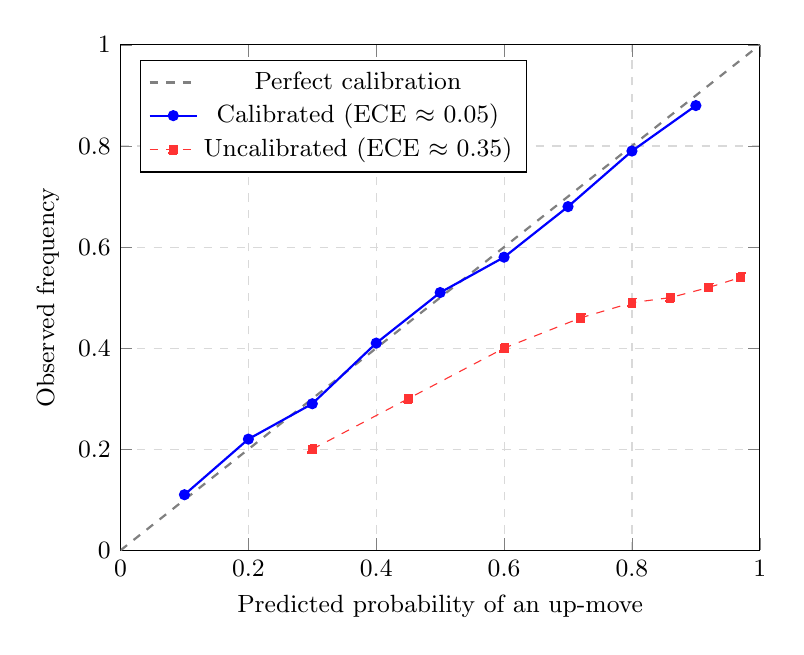
\begin{tikzpicture}
\begin{axis}[
  width=0.8\textwidth, height=80mm,
  xlabel={Predicted probability of an up-move},
  ylabel={Observed frequency},
  xmin=0,xmax=1,ymin=0,ymax=1,
  grid=major,grid style={dashed,gray!30},
  legend pos=north west,legend style={font=\small},
  tick label style={font=\small},label style={font=\small}
]
\addplot[gray,dashed,thick] coordinates{(0,0)(1,1)};
\addlegendentry{Perfect calibration}
\addplot[blue,mark=*,mark size=1.6pt,thick] coordinates{
  (0.10,0.11)(0.20,0.22)(0.30,0.29)(0.40,0.41)
  (0.50,0.51)(0.60,0.58)(0.70,0.68)(0.80,0.79)(0.90,0.88)};
\addlegendentry{Calibrated (ECE $\approx$ 0.05)}
\addplot[red!80,mark=square*,mark size=1.6pt,dashed] coordinates{
  (0.30,0.20)(0.45,0.30)(0.60,0.40)(0.72,0.46)
  (0.80,0.49)(0.86,0.50)(0.92,0.52)(0.97,0.54)};
\addlegendentry{Uncalibrated (ECE $\approx$ 0.35)}
\end{axis}
\end{tikzpicture}
\caption{Reliability diagram before and after the three-stage calibration
(see Figure Captions).}
\label{fig:calib}
\end{figure}

\end{document}
